%% The following is a directive for TeXShop to indicate the main file
%%!TEX root = diss.tex

\chapter{Conclusion}
\label{ch:conc}

%%%%%

Molecular emission was successfully detected in our experiments, demonstrating that our system is capable of \ac{STML} experiments. In our studies of \ac{ZnPc}, broad molecular photoluminescence signals were observed at positive biases. The signals differ from previously reported \ac{STML} on the molecule at negative biases. As the molecules were more mobile when scanned at high positive bias, it is possible that the stability and motion of the molecules on the surface can affect the photon emission process. Other explanations include the presence of an alternate pathway for exciton generation, such as photon-mediated, or the tunnelling into higher energy unoccupied orbitals, such as LUMO+1. Signals detected in our study of \ac{PTCDA} are the first reported single molecule emission on uncharged \ac{PTCDA}. Similar to the emission detected on \ac{ZnPc}, the experiment was conducted at positive bias, and the detected emission peak was broad.

The effects of fluorination on the photoluminescence of ZnPc were studied through the \ac{SPM} of \ch{F8ZnPc}. \ac{STML} was detected at a bias of \SI{-2.5}{V}, similar to parameters of previously reported \ac{STML} on ZnPc. However, photon emission detected on \ch{F8ZnPc} varied in wavelength from 630\SI{-640}{nm} for different \ch{F8ZnPc} on the surface. \ac{STM} scans at negative biases revealed a variety of topographically different molecules, and point \ac{STS} on the molecules showed differing \ac{LDOS} resonances for the molecules. Repeated sample preparation and replacing of molecules ruled out the presence of degraded molecule, and the switching between molecular species through tip manipulation seemed to indicate that the variety was due to changes in surface adsorption of the molecules. Molecules with smaller band gaps in the \ac{STS} spectra produced lower energy emission peaks in the \ac{STML} spectra, demonstrating correlation between the shifts in electronic states and the optical gap of formed excitons.

After a full system bake-out, a new sample was produced, and the variety of \ch{F8ZnPc} was observed again. However, the sample was noticeably different, with fewer defects on the NaCl bilayers, and new types of \ch{F8ZnPc} observed than those of the sample used for \ac{STML}. Regardless, the different types of molecules were categorized by \ac{STS} spectral features, \ac{STM} topographic differences, and relative positions on the NaCl lattice. We conclude that the presence of the fluorines in \ch{F8ZnPc} stabilize certain adsorption geometries not observed for ZnPc. These changes in conformation and interactions with the substrate can affect the electronic and optical properties of the molecules.

In our study of HMAT derivatives, using pixel-by-pixel \ac{STS}, sub-molecular images of the molecular orbitals for each HMAT molecule were generated. We find that the HOMO was localized around the donor complexes, the HMAT groups, of the molecules, while the LUMO was localized around the acceptor complexes. With the functionalization of increasingly electronegative acceptor groups, the band gaps obtained through \ac{STS} were observed to decrease, demonstrating the tuning of electron energy levels in molecules through chemical design. The results observed in our experiments qualitatively agree with DFT calculations of the HMAT derivatives in gas phase. \ac{STML} experiments were attempted for the HMAT derivatives, however, due to the large band gap, high biases would be required to generate excitons in the material, which could break or move the molecules on the surface.




\section{Future directions}

% talk about the new windows
% talk about using a photomultiplier
% talk about mounting a proper height crystal of Au(111).
With the installation of wider bandwidth filter windows in our \ac{SPM}, reproduction of experiments described in the thesis may be worthwhile, as the cutoff and broadening effects of the IR Filter windows would be eliminated in future \ac{STML} experiments. For further improvements, all samples used for \ac{STML} should be at the correct height for maximum emission collection by the \textit{in situ} lens. Additionally, a photomultiplier tube can be installed in place of the spectrometer. With software improvements, the position of the tip can be synchronized with the photomultiplier tube signal to give sub-molecular photon maps of molecular photoluminescence.

The broad emission peaks in our positive bias \ac{STML} studies remain unexplained. In the thesis, several explanations have been provided, but additional experimentation may reveal the exact emission mechanism, and explain the divergences from previously reported results. In particular, the hypothesis of excitons formed by tunnelling into the LUMO+1 of uncharged \ac{PTCDA} may be tested by mapping out the LUMO+1 using bias dependent \ac{STML}. To test whether the stability of molecules at higher biases have an effect on the observed emission, \ac{STML} experiments can be carried out on \ac{ZnPc} or \ac{PTCDA} ``anchored" to features such as defects or step edges on the surface. 

Future experiments can be directed to the study of systems of organic semiconductors on the surface. By annealing the sample, molecules can self-assemble into dimers. The effects of molecule-molecule interactions, such as polarization and charge transfer, on the formed exciton can be examined by \ac{STML} on the dimerized molecules. Additionally, heterodimers of different molecules, such as PTCDA-ZnPc or ZnPc-\ch{F8ZnPc}, can be studied as simplified models of device heterojunctions. Successful formation of ZnPc-\ch{F8ZnPc} dimers have already been demonstrated on (2ML)NaCl/Au(111), as seen in \autoref{fig:conclusion:f8znpc_znpc_dimer}. 

\begin{figure}[H]
    \centering
    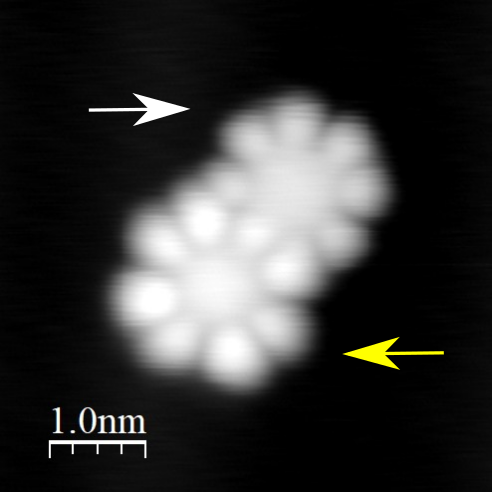
\includegraphics[width=0.5\textwidth]{pictures/f8znpc_znpc_dimer_arrows.png}
    \caption{\sloppy STM image of dimerized \ch{F8ZnPc} and ZnPc on (2ML)NaCl/\-Au(111) (\stmparams{5}{5}{-2.5}{5}). The white and yellow arrows indicate the \ch{F8ZnPc} and ZnPc, respectively.}
    \label{fig:conclusion:f8znpc_znpc_dimer}
\end{figure}

In our study of \ch{F8ZnPc}, we have demonstrated that adsorption geometry can change the electronic structure of the molecule. Separately, we have demonstrated that the change in electronic structure correlates with change in the exciton optical gap. Due to variations in the samples, we cannot make conclusions between the types of \ch{F8ZnPc} observed and the \ac{STML}. A future direction would be to examine the molecules on cleaner NaCl bilayers with the Ag tip, giving simultaneous \ac{STS} and \ac{STML} measurements. Furthermore, theoretical simulations of adsorption geometries of \ch{F8ZnPc} on (2ML)NaCl/Ag(111) may give information on the role of the fluorine atoms on the conformation of the molecule, and resulting changes in molecular orbitals.

Future experiments on the HMAT derivatives are limited due to the incompatibility of the molecules to \ac{SPM} on insulating layers on metallic substrates. Nonetheless, experiments on the HMAT molecules have revealed the necessary properties of candidate molecules for further \ac{STML} experiments, such as a planar structure, and HOMO/LUMO states that do not lie further than \SI{3}{V} from the Fermi level. With an appropriate molecular, the effects of chemical design on the excitonic emission can be studied in future \ac{STML} experiments.





                                    